\section*{Abstract}
In this paper we will study the magnetopause using real data from the Cluster satellites. We will identify the times that the satellite crossed the magnetopause, estimate the normal to the magnetopause and estimate the current density at the magnetopause. These results will be compared to ideal values and discussed.

\section*{Exercise 1}
	In this exercise, example 2.1.1 was implemented using the magnetic field data that was provided. The equations below show the matrices D and V, where the diagonals of D are the eigenvalues and the columns of V are the corresponding eigenvectors.
   \begin{multicols}{2}
    \begin{equation}
    	D =
    	\begin{bmatrix}
        	7.1 & 0 & 0 \\
             0  & 137.9 & 0 \\
             0  &  0 & 1012.9 \\
         \end{bmatrix}
     \end{equation}
     
     \begin{equation}
         V =
         \begin{bmatrix}
         	0.8671 & 0.2886 & -0.4061 \\
   			-0.4978 & 0.5326 & -0.6845 \\
    		 0.0187 & 0.7957 & 0.6054 \\
          \end{bmatrix}
      \end{equation}
    \end{multicols}
Here, the smallest eigenvalue $\bf{e} = 7.1$ corresponds to $\bf{n} = [0.8671 -0.4978 -0.0187]$.

\section*{Exercise 2}
	Based on the Cluster data, the proton data and magnetic field data were plotted against time as seen below in \ref{fig:protdata} and \ref{fig:magdata}. The plasma beta was calculated according to the given formula \ref{eq:beta}.
    
    \begin{equation}
    \beta = \frac{n (2T_{\bot} + T_{\parallel} ) * 0.5}{B^2 / (0.5 \mu_0)}
    \label{eq:beta}
    \end{equation}

    
    \begin{figure}[h!]
    	\centering
            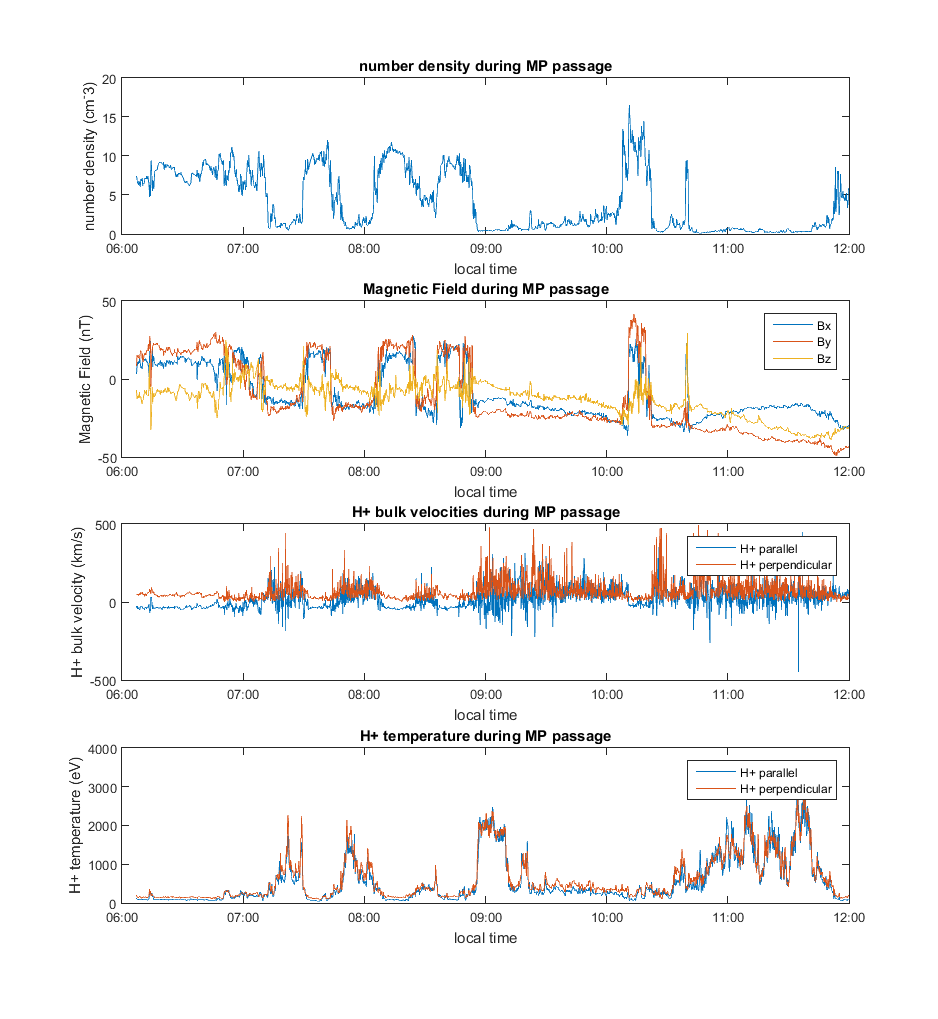
\includegraphics[scale=0.6]{images/otherPlots.png}
            \caption{Proton Data Variation over Time}
            \label{fig:protdata}
	\end{figure}
	\begin{figure}[h!]
    		\centering
			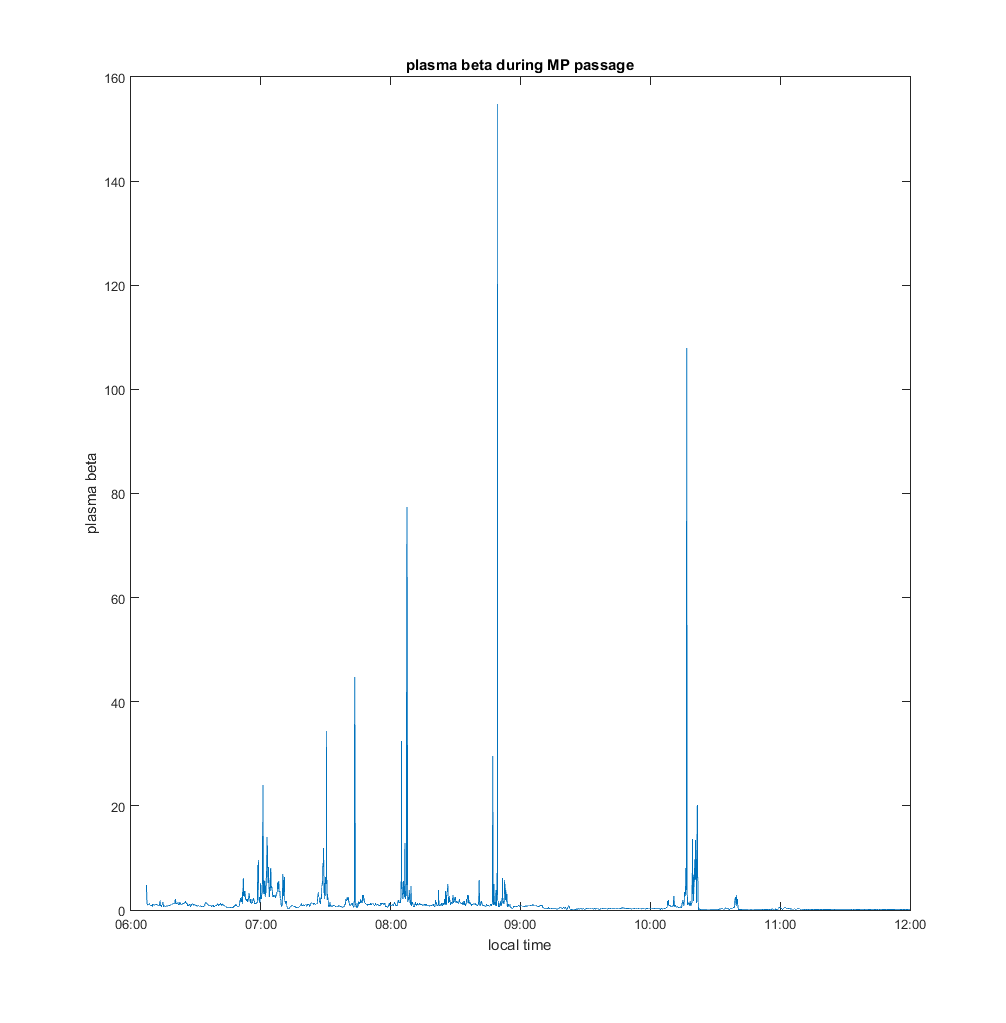
\includegraphics[scale=0.6]{images/plasma_Beta.png}
            \caption{Plasma Beta Variaion over Time}
            \label{fig:magdata}
    \end{figure}
\clearpage
	\subsection*{Question 1}
    	The magnetosheath can be distinguished from the magnetosphere by finding the regions where the the ion velocity decreases and the ion density increases. These regions of the graph are where the spacecraft moves from the magnetosphere to the magnetosheath. Another way to distinguish the two is by looking at the energy of the particles, which tend to decrease when crossing from magnetosphere to magnetosheath.
        
%Crossings in plots: "We identify a magnetopause crossing when we see a decrease / increase of the plasma density and velocity at the same time and simultaneously an increase / decrease of the temperature."
        
    \subsection*{Question 2}
     We observe 10 Magnetopause Crossings, there is a very short spike occurring between 10:35 and 10:43 that we are not taking into account as we believe it is an anomaly due to the short time and low peak height.
     \Cref{tab:crossings} shows the timeslots during which Magnetopause crossings occur.
     
\begin{table}[h!]
\centering
\caption{Timeslots where Magnetopause crossings occur}
\label{tab:crossings}
\begin{tabular}{llllllllll}
07:10-07:13 & 07:28-07:31 & 07:43-07:46 & 08:04-08:07 & 08:22-08:25\\  08:35-08:38 & 08:52-08:56 & 10:07-10:09 & 10:21-10:23 & 11:52-11:55
\end{tabular}
\end{table}
    
\subsection*{Question 3}
With the MVAB method, the normal for the magnetopause of each crossing was calculated. In a similar way to the first exercise, the eigenvector with respect to the smallest eigenvalue gives the normal to the magnetopause normal for each crossing.\\
\Cref{table:xyzdata} lists the normal vectors for each crossing. Each change in polarity of the vectors indicates a crossing. The coordinate data indicates that during the daytime the satellite is in the southern hemisphere (positive $x$ and negative $z \text(and) y$). The estimated normal directions are very close to the expected value. The direction of every second crossing is the same which corroborates the validity of the data.

\begin{table}[H]
\centering
\caption{Magnetopause normal vectors.}
\begin{tabular}{ |c||c c c| }
    \hline
    Crossing nr. & $x$ & $y$ & $z$  \\ \hline \hline
  1 &  0.7456 &   0.1559  &  0.6479 \\ \hline
  2 &  0.6726  & -0.7112  & -0.2044 \\ \hline
  3 &  0.0475 &   0.0732  &  0.9962 \\ \hline
  4 &  0.4679  &-0.6427  & -0.6066 \\ \hline
  5 &  0.8199 &   0.3059 &  -0.4839 \\ \hline
  6 &  0.7188  & -0.6952  &  0.0041 \\ \hline
  7 &  0.8354   &-0.0857  &  0.5428 \\ \hline
  8 & -0.0848   & 0.5236  & -0.8477 \\ \hline
  9 &  0.7445  & -0.5072  & -0.4342 \\ \hline
  10 & -0.8436  & -0.0793  & -0.5311 \\ \hline
   
    \end{tabular}
\label{table:xyzdata}
\end{table}

\subsection*{Question 4}
   By comparing the values given in \textit{Outer Magnetospheric Boundaries: Cluster Results}(G. Paschmann et. al. (2005)) chap.8.3.3 to our values, we can see that the values we get are in the same magnitude, but have a slightly higher range. Their lowest average value of 0.01 $\mu A m^{-2}$ is comparable to our 10$^{th}$ crossing, whereas the largest average value of 0.3 $\mu A m^{-2}$ is a lot lower than our highest value of 1.5231$\mu A m^{-2}$ during crossing 7. Thus, the mean value of the average currents is 0.05$\mu A m^{-2}$, which is almost a magnitude lower than our mean value of 0.8497$\mu A m^{-2}$.
   
Despite this our current densities seem to be reasonable because they have a similar magnitude to the average values.

 \begin{table}[H]
\centering
\caption{absolute current density for crossings}
\begin{tabular}{ |c||c| }
    \hline
    Crossing nr. & current density ($\mu Am^{-2}$)\\ \hline \hline
  1 &  0.5186  \\ \hline
  2 &  0.5332 \\ \hline
  3 &  0.8980  \\ \hline
  4 &  0.9987  \\ \hline
  5 &  0.5080 \\ \hline
  6 &  1.4680  \\ \hline
  7 &  1.5231  \\ \hline
  8 &  0.7961  \\ \hline
  9 &  1.2408  \\ \hline
  10 & 0.0127 \\ \hline
   
    \end{tabular}
\label{table:currents}

\section*{Conclusion}
In this experiment we have used matlab to analyze a set of real data from the cluster satellites. We distinguished the magnetosphere from the magnetosheath and used this information to identify when the satellite crossed from one area to the other. We also estimated the normal for the magnetopause at each crossing and compared our results to ideal results from a textbook. Finally we estimated the average current density at the crossing to be 0.8497$\mu A m^{-2}$ and compared it to typical magnetopause currents.
\end{table}

